\chapter[Ecuaciones de la Dinámica]{Ecuaciones fundamentales de la Dinámica de los Fluidos}
\section{Introducción}
	
	La Mecánica de los fluidos viene determinada por \textcolor{red}{3
		leyes básicas}\footnote{Algunos autores, como \cite{Shames2003} toman en consideración también
		la Segunda Ley de la Termodinámica}
	
	\begin{itemize}
		\item \textcolor{black}{El principio de }\textcolor{red}{conservación de
			la masa}\textcolor{black}{. La masa de un sistema fluido se mantiene
			constante independientemente de su posición o forma. }
		\item \textcolor{black}{La ley de }\textcolor{red}{conservación de la cantidad
			de movimiento}\textcolor{black}{. La variación de la cantidad de movimiento
			de un sistema fluido es igual a la suma total de la fuerzas externas
			que actúan sobre él. }
		\item \textcolor{black}{La ley de }\textcolor{red}{conservación de la energía}\textcolor{black}{.
			Es, básicamente, la Primera Ley de la Termodinámica. La variación
			de la energía de un sistema fluido (energía interna + energía cinética)
			es igual al trabajo realizado por todos las fuerzas externas más el
			calor recibido por conducción y/o radiación. }
	\end{itemize}
	A estos principios hay que añadir las \textcolor{blue}{leyes constitutivas},
	como la ley de viscosidad de Newton, o la ley de los gases perfectos. 


\section{Formulación integral y diferencial}

	
	Existen dos enfoques para los problemas de Mecánica de Fluidos: 
	\begin{itemize}
		\item \textcolor{red}{Formulación diferencial}. Se consideran volumenes
		elementales de fluido y las ecuaciones que gobiernan su comportamiento.
		Para resolver los problemas con este planteamiento es necesario conocer
		las condiciones iniciales en todo el dominio y las condiciones de
		contorno en todos los límites del mismo. 
		\item \textcolor{red}{Formulación integral}. Se trabaja directamente sobre
		volumenes de fluido macroscópicos, denominados \textcolor{blue}{volúmenes
			de control}. Las ecuaciones son promediadas en el volumen de control
		y sobre su frontera, denominada \textcolor{blue}{superficie de control}. 
	\end{itemize}
	Para la mayoría de los problemas de Ingeniería ( o, por lo menos,
	para una primera aproximación) es suficiente con la formulación integral\footnote{La formulación diferencial es
		más general, y permite determinar detalles del flujo. Es posible extraer
		los resultados de la formulación integral a partir de los de la diferencial,
		pero no al contrario.}.


\subsection{Sistema y volumen de control}

	
	Un \textcolor{blue}{sistema de control} posee una cantidad definida
	de materia. Su volumen, y, por lo tanto, su densidad, así como otras
	magnitudes físicas pueden cambiar, pero no la cantidad de masa. En
	mecánica de sólidos se suele emplear el sistema de control como enfoque
	de trabajo.
	
	En Mecánica de Fluidos, es conveniente usar el enfoque de \textcolor{blue}{volúmen
		de control}, que se establece en el espacio, sin relación con una
	cierta cantidad de materia. Este volumen puede ser estático o no,
	y puede cambiar tanto de posición como de tamaño.
	
	La diferencia entre sistema y volumen de control se puede relacionar
	con la diferencia entre los puntos de vista Lagrangiano y Euleriano,
	ya que un sistema de control siempre sigue el movimiento de las partículas
	que lo componen.


\subsection{El teorema de arrastre de Reynolds}

	
	Dado que las ecuaciones de mecánica y termodinámica se refieren a
	sistemas de control, es necesario deducirlas para el caso en que las
	aplicamos sobre volúmenes de control.
	
	Consideremos un volumen de control y un sistema de control que, en
	un instante determinado $t$, coinciden en el espacio. El volumen
	de control $VC$ está estacionario, mientras que el sistema de control
	$V$ se mueve con el flujo.
	
		En el instante $t+\delta t$
				el sistema de control se encuentra en una posición ligeramente desplazada
				respecto al volumen. Incluso puede que haya cambiado su volumen, si
				el flujo es compresible
	
\begin{center}
	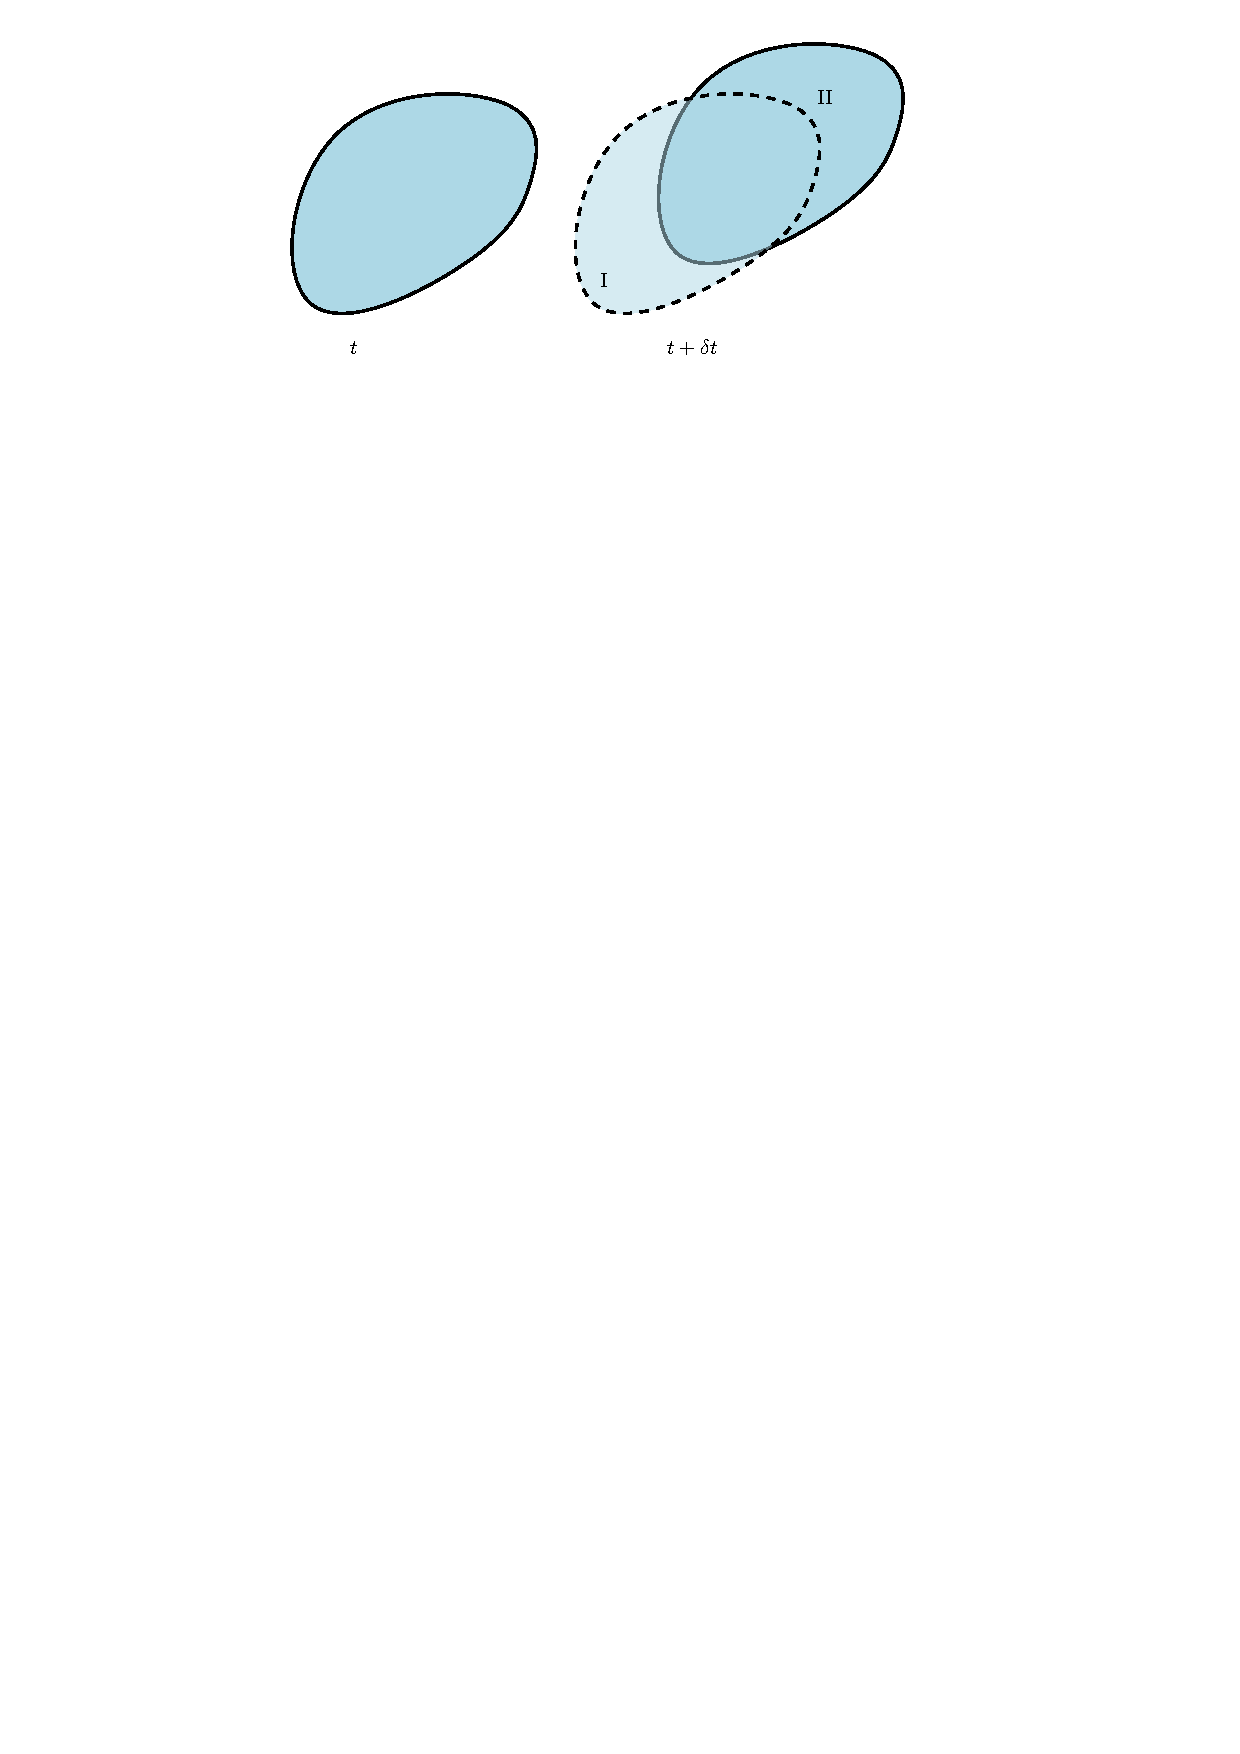
\includegraphics[width=0.7\linewidth]{TeX_files/chapter04-Dinamica/VC}
\end{center}


Consideremos una cierta magnitud extensiva $F$, y $f$ la misma por
unidad de masa, de forma que


\begin{equation}
	F=\int_{V}\rho f\,\text{d}V
\end{equation}


Consideremos la notación: \textcolor{black}{\scriptsize{}
	\begin{eqnarray*}
		F_{t} & : & \text{el valor de \ensuremath{F} para el sistema de control en el instante \ensuremath{t}}\\
		F_{t^{+}} & : & \text{el valor de \ensuremath{F} para el sistema de control en el instante \ensuremath{t+\delta t}}\\
		F'_{t} & : & \text{el valor de \ensuremath{F} para el volumen de control en el instante \ensuremath{t}}\\
		F'_{t^{+}} & : & \text{el valor de \ensuremath{F} para el volumen de control en el instante \ensuremath{t+\delta t}}\\
		F_{s} & : & \text{Cantidad de \ensuremath{F} que abandona el volumen de control en el intervalo \ensuremath{\Delta t} (a través de I)}\\
		F_{e} & : & \text{Cantidad de \ensuremath{F} que entra en el volumen de control en el intervalo \ensuremath{\Delta t} (a través de II)}
	\end{eqnarray*}
}{\scriptsize\par}

Evidentemente, 
\[
F_{t}=F'_{t}
\]


	
	Las variaciones de $F$ en el sistema de control y en el volumen de
	control son, respectivamente, 
	\begin{eqnarray*}
		\delta F & = & F_{t^{+}}-F_{t}\\
		\delta F' & = & F'_{t^{+}}-F'_{t}
	\end{eqnarray*}
	y, por otro lado, 
	\[
	F_{t^{+}}=F'_{t^{+}}+F_{s}-F_{e},
	\]
	de forma que 
	\[
	\delta F=\delta F'+F_{s}-F_{e}
	\]
	
	Dividiendo por $\delta t$ y haciendo el límite $\delta t\rightarrow0$,
	obtenemos 
	\[
	\deriv{F}{t}=\deriv{F'}{t}+\lim_{\delta t\rightarrow0}\frac{F_{s}-F_{e}}{\delta t}
	\]
	

	
	Por definición, el último término es el flujo de $F$ a través de
	la frontera de $VC$, que, como hemos definido en temas anteriores,
	
	\[
	\lim_{\delta t\rightarrow0}\frac{F_{s}-F_{e}}{\delta t}=\Phi_{F}=\oint_{SC}\rho f\vec{u}_{r}\cdot\text{d}\vec{S}
	\]
	
	\[
	\deriv{F}{t}=\deriv{F'}{t}+\oint_{SC}\rho f\vec{u}_{r}\cdot\text{d}\vec{S}
	\]
	

\begin{equation}
		\Rightarrow\boxed{\deriv{F}{t}=\deriv{\phantom{F}}{t}\int_{VC}\rho f\,\text{d}V+\oint_{SC}\rho f\vec{u}_{r}\cdot\text{d}\vec{S}}
\end{equation}
	,donde $\vec{u}_{r}$ es la velocidad del flujo relativa a la Superficie
	de Control.\\
	

	
	Otra forma de expresarlo es, usando el Teorema de Leibniz \cite[Sección 3.6]{Kundu2012}
	
\begin{equation}
		\boxed{\deriv{F}{t}=\int_{VC}\dparc{\rho f}{t}\,\text{d}V+\oint_{SC}\rho f\vec{u}\cdot\text{d}\vec{S}}
\end{equation}
	,donde $\vec{u}$ es ahora la velocidad absoluta. Si el VC no se mueve
	ni se deforma, $\vec{u}=\vec{u}_{r}$. 
	
	Se puede usar el Teorema de la Divergencia para transformar la integral
	de superficie en una integral de volumen, de forma que
	
	\[
	\deriv{F}{t}=\int_{VC}\dparc{\rho f}{t}\,\text{d}V+\int_{VC}\vec{\nabla}\cdot\left(\rho f\vec{u}\right)\text{d}V
	\]
	
	\[
	\Rightarrow\deriv{F}{t}=\int_{VC}\left[\dparc{\rho f}{t}+\vec{\nabla}\cdot\left(\rho f\vec{u}\right)\right]\text{d}V
	\]
	
\section{Ecuación integral de conservación de la masa}

	
	En este caso, $F=m$ y $f=1$. Por definición de sistema físico, $\deriv{m}{t}=0$,
	de forma que 
	\[
	\int_{VC}\dparc{\rho}{t}\,\text{d}V+\oint_{SC}\rho\vec{u}\cdot\text{d}\vec{S}=0
	\]
	
	\[
	\Rightarrow\,\boxed{\int_{VC}\dparc\rho t\,\dif V=-\oint_{SC}\rho\vec{u}\cdot\dif\vec{S}}
	\]
	
	Interpretación física: \textbf{\textcolor{red}{En un Volumen de Control,
			la variación local de la masa únicamente puede ser debida a un flujo
			de masa a través del contorno.}} 

	
	Simplicaciones de la ecuación integral de conservación de la masa
	\begin{itemize}
		\item Si el flujo es \textcolor{blue}{estacionario} en el interior del VC,
		entonces $\dparc{\rho}{t}=0$ y
		\[
		\oint_{SC}\rho\vec{u}\cdot\text{d}\vec{S}=0
		\]
		
		\item Si el flujo es \textcolor{blue}{incompresible}, entonces la densidad
		es constante en todo el VC, de forma que
		\[
		\int_{VC}\dparc\rho t\,\text{d}V=-\rho\oint_{SC}\vec{u}\cdot\text{d}\vec{S}
		\]
		
		\item Si se cumplen las dos condiciones y el flujo es \textcolor{blue}{incompresible
			y estacionario},
		\[
		\oint_{SC}\vec{u}\cdot\text{d}\vec{S}=0
		\]
	\end{itemize}


\subsection{Definición de velocidad media}

	
	Consideremos como caso simple un fluido incompresible circulando por
	una tubería. La sección de la tubería es $S$, y el flujo se puede
	considerar en todos los puntos axial, de forma que el caudal se calcula
	con 
	\[
	Q=\int_{S}u\text{d}S
	\]
	
	La \textcolor{red}{velocidad media} se define como la velocidad uniforme
	que debería tener el flujo para que el caudal fuese el mismo, $Q=\mean{u}S$.
	De aqui, 
	\[
	\mean{u}=\frac{1}{S}\int_{S}u\text{d}S
	\]
	\\
	Un documento muy interesante para estudiar la forma integral de la
	conservación de la masa, es el publicado en 2001 por el prof. Sonin,
	del MIT, disponible \href{http://web.mit.edu/2.25/www/pdf/cv.pdf}{aqui}.


\section{Ecuación diferencial de conservación de la masa}

	
	Aplicando el Teorema de la Divergencia a la forma integral, para un
	Volumen de Control estacionario, se obtiene 
	\[
	\int_{VC}\left[\dparc\rho t+\vec{\nabla}\cdot\left(\rho\vec{u}\right)\right]\text{d}V=0
	\]
	
	Como esto debe cumplirse para cualquier VC, obtenemos la forma diferencial
	de la conservación de la masa: 
	\[
	\dparc\rho t+\vec{\nabla}\cdot\left(\rho\vec{u}\right)=0
	\]
	
	En forma de componentes: 
	\[
	\dparc{\rho}{t}+\dparc{}{x_{i}}\left(\rho u_{i}\right)=0
	\]
	

\subsection{Líneas de corriente}

	
	Para un \textcolor{blue}{fluido incompresible}: 
	\[
	\vec{\nabla}\cdot\vec{u}=0
	\]
	
	\[
	\text{Flujo 2D}\quad\rightarrow\quad\dparc{u}{x}+\dparc{v}{y}=0
	\]
	
	Consideremos una función $\psi(x,y)$ que cumple 
	\[
	u=\dparc{\psi}{y}\quad;\quad v=-\dparc{\psi}{x}
	\]
	
	Entonces la ecuación de continuidad se cumple de forma exacta, ya
	que 
	\[
	\dparc{\phantom{x}}{x}\left(\dparc{\psi}{y}\right)+\dparc{\phantom{y}}{y}\left(-\dparc{\psi}{x}\right)\equiv0
	\]
	

	
	$\psi(x,y)$ es la \textcolor{red}{función de corriente}.
	
	Las líneas $\psi(x,y)=\psi_{i}=\text{cte}$ son las \textcolor{red}{líneas
		de corriente} y cumplen que 
	\[
	\text{d}\psi=0\Rightarrow\dparc{\psi}{x}\text{d}x+\dparc{\psi}{y}\text{d}y=0
	\]
	\[
	\Rightarrow-v\text{d}x+u\text{d}y=0\,\Rightarrow\,\frac{\text{d}x}{u}=\frac{\text{d}y}{v}
	\]
	
	es decir, son \emph{tangentes a $\vec{u}$} en todos los puntos

	
Interpretación física:
		
		Flujo bidimensional. Para una profundidad unidad:
		
\begin{center}
	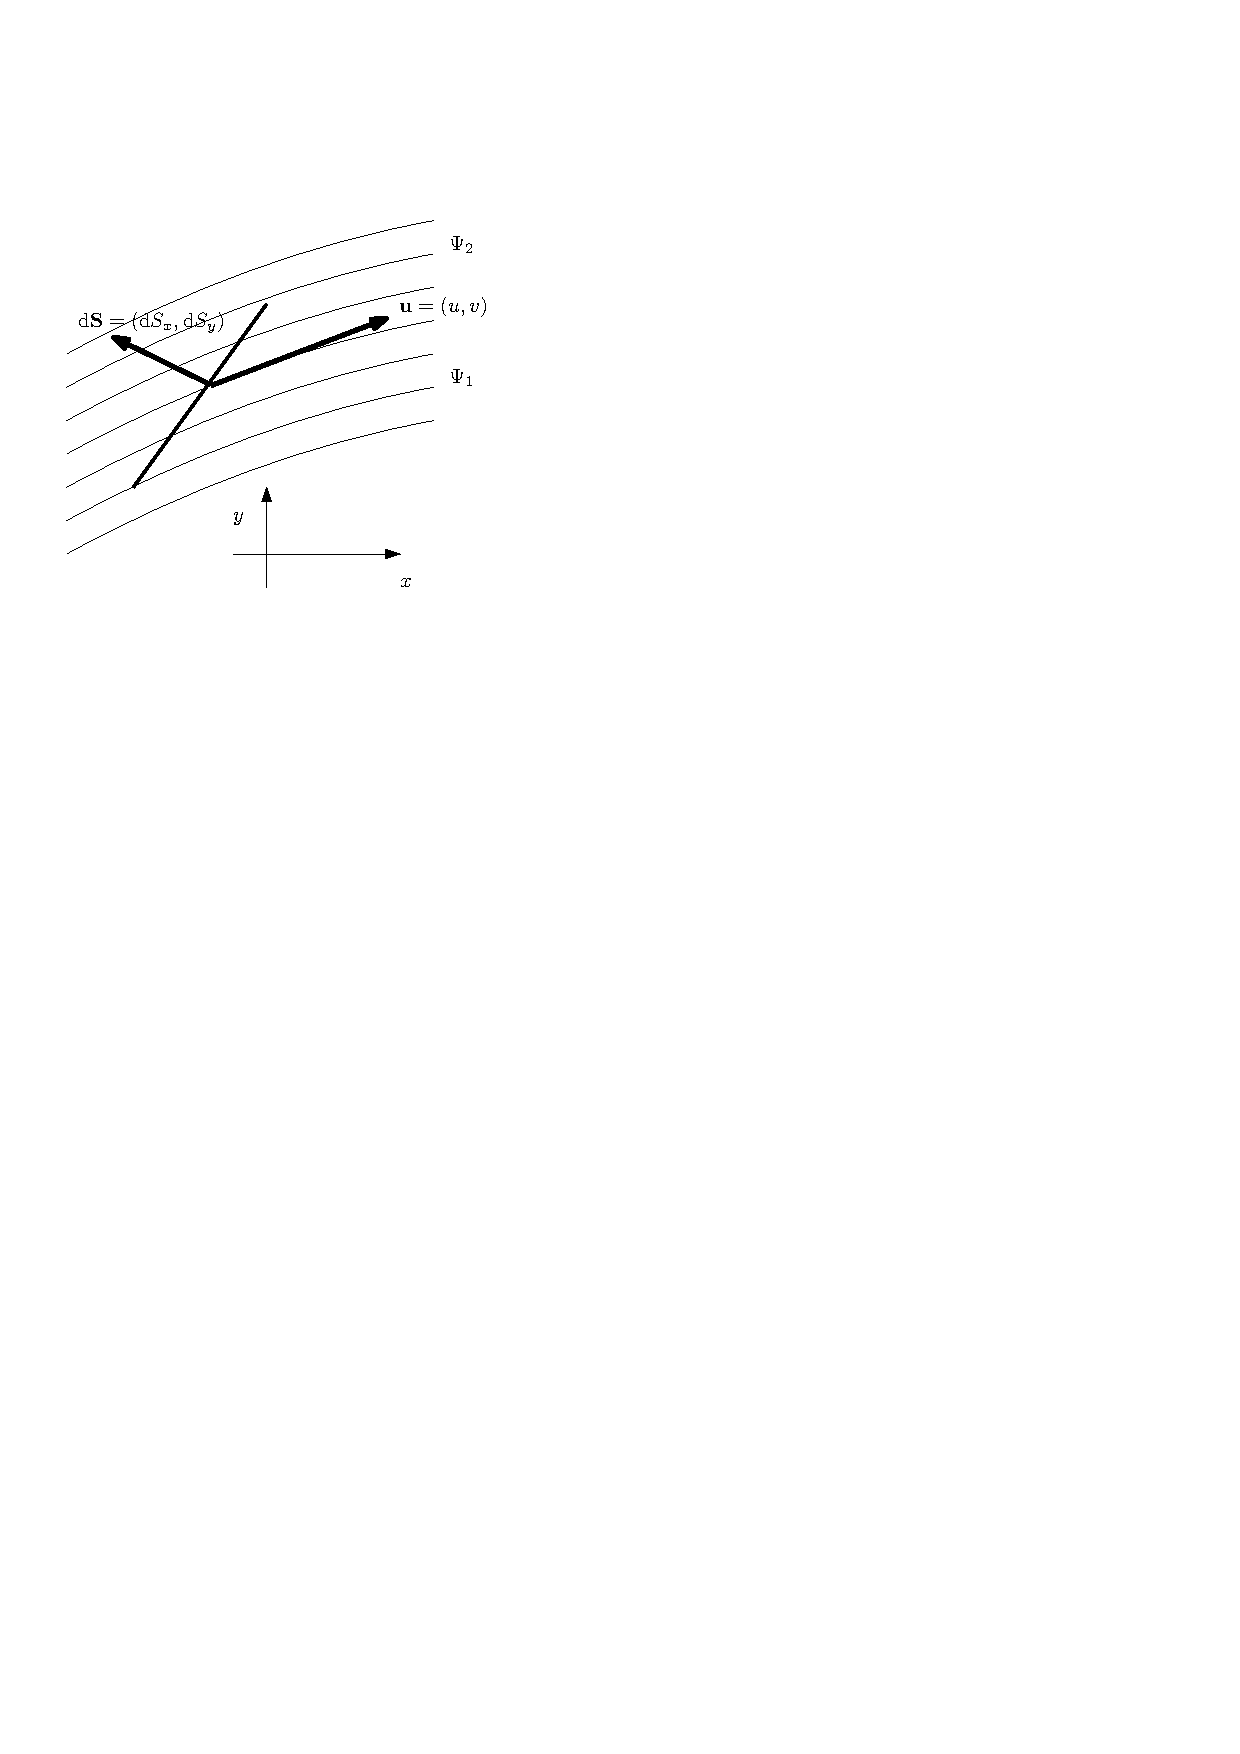
\includegraphics[width=0.4\linewidth]{TeX_files/chapter04-Dinamica/Phi1}
\end{center}

%			\input{interp_fisica_f_corr_2.pdftex_t}%
%		\end{minipage}\hfill{}%

			\begin{align*}
				dQ & =\vec{u}\cdot\text{d}\vec{S}\\
				 & =  \left(\begin{array}{cc}
					u & v\end{array}\right)\left(\begin{array}{c}
					\text{d}S_{x}\\
					\text{d}S_{y}
				\end{array}\right)\\
				& = \left(\begin{array}{cc}
					\dparc{\psi}{y} & -\dparc{\psi}{x}\end{array}\right)\left(\begin{array}{c}
					\text{d}y\\
					-\text{d}x
				\end{array}\right)(\times1)\\
				& =  \dparc{\psi}{y}\text{d}y+\dparc{\psi}{x}\text{d}x=\dif\psi\\
				\Rightarrow & \; Q=\psi_{2}-\psi_{1}
			\end{align*}


	
\subsection*{Actividad 1:}
		\[
		\vec{u}(x,y)=u(x,y)\,\vec{\imath}+v(x,y)\,\vec{\jmath}
		\]
		con $u(x,y)=a(x^{2}-y^{2})$. ?`Como tiene que ser de forma general
		$v(x,y)$ para que el flujo sea incompresible?
		
		Calcular la función de corriente y dibujar las lineas de corriente
		para el caso más simple.

